\documentclass[10pt]{article}
\usepackage[utf8]{inputenc}
\usepackage{listings}
\usepackage{float}
\usepackage{graphicx}
\usepackage{fullpage}
\usepackage{caption}
\usepackage{subcaption}
\usepackage{amsmath}

%\renewcommand{\thesubsection}{\arabic{subsection}}
\renewcommand{\thesubsubsection}{\alph{subsubsection}}

\title{Pattern Recognition practical 2}
\author{Maikel Withagen (s1867733) \and Steven Bosch (s1861948)}
\date{\today}
\lstset{frame=single, numbers=left,language=Matlab,basicstyle=\small, title=\lstname}

\begin{document}

\maketitle

\section{Covariance matrix}
\subsection{}
Using the code given in the appendix we get the following mean vector:
\begin{equation}
    \begin{bmatrix}
      5.8000 \\
      5.0000 \\
      6.2000
    \end{bmatrix}
\end{equation}
And the following covariance matrix is yielded:

  \begin{equation}
    \begin{bmatrix}
      3.2000  &  0.2500 &  -0.4500 \\
      0.2500  &  2.5000 &  -3.7500 \\
    -0.4500 &  -3.7500 &   5.7000
    \end{bmatrix}
\end{equation}

\subsection{}
We computed the following probability densities:
\begin{lstlisting}
>> mvnpdf([5;5;6], mean1, cov1)
ans =    0.0543
>> mvnpdf([3;5;7], mean1, cov1)
ans =   6.1287e-04
>> mvnpdf([4;6.5;1], mean1, cov1)
ans =   7.0300e-29
\end{lstlisting}

\section{Covariance matrix, analytically}
Every element in the covariance matrix is determined by:
\begin{equation}
\sigma_{ij} = \frac{1}{n-1} \sum_{n=1}^{N} (x_{in}-\mu_{i})(x_{jn} - \mu_{j})
\end{equation}
Since $n=2$ for all the covariance matrices calculated below, we leave that factor out (since $\frac{1}{2-1}=1$).

\subsection{}
Element 1,1:
\begin{align}
\sigma_{1,1} & = (a-\frac{a+c}{2})^2+(c-\frac{a+c}{2})^2 \\
& = (\frac{a-c}{2})^2 + (\frac{c-a}{2})^2 \\
& = \frac{1}{4}(a-c)^2 + \frac{1}{4}(c-a)^2 \\
& = \frac{1}{2}(a-c)^2
\end{align}
Similarly for $\sigma_{2,2}$ we get $\frac{1}{2}(b-d)^2$.
For the other two elements, $cov(1,2)$ and $cov(2,1)$ which are the same, we get the following:
\begin{align}
\sigma(1,2) & = ((a-\frac{a+c}{2})(b-\frac{b+d}{2})+(c-\frac{a+c}{2})(d-\frac{b+d}{2})) \\
& = (\frac{a-c}{2}) (\frac{b-d}{2}) + (\frac{c-a}{2}) (\frac{d-b}{2}) \\
& = \frac{(a-c)(b-d) + (c-a)(d-b)}{4} \\
& = \frac{2ab - 2ad - 2bc + 2cd}{4} \\
& = \frac{1}{2} (a-c)(b-d)
\end{align}
This results in the following covariance matrix:
\begin{equation}
    \begin{bmatrix}
      \frac{1}{2}(a-c)^2 & \frac{1}{2} (a-c)(b-d)\\
      \frac{1}{2} (a-c)(b-d) & \frac{1}{2}(b-d)^2
    \end{bmatrix}
\end{equation}

\subsection{}
Element 1,1:
\begin{align}
\sigma_{1,1} & = (a+k-\frac{a+c+2k}{2})^2+(c+k-\frac{a+c+2k}{2})^2 \\
& = (\frac{a-c}{2})^2 + (\frac{c-a}{2})^2 \\
& = \frac{1}{4}(a-c)^2 + \frac{1}{4}(c-a)^2 \\
& = \frac{1}{2}(a-c)^2
\end{align}
As we can see, the $k$s are all removed in the simplification, due to writing sums like $a+k$ as the fraction $\frac{2a+2k}{2}$ and subtracting fractions with $2k$ in the numerator, resulting in the $k$s being removed.
Again similarly for $\sigma_{2,2}$ we get $\frac{1}{2}(b-d)^2$.
For the other two elements, $cov(1,2)$ and $cov(2,1)$ we get the following (the $k$s are removed in the simplification process again):

\begin{align}
\sigma(1,2) & = ((a+k-\frac{a+c+2k}{2})(b+k-\frac{b+d+2k}{2})+(c+k-\frac{a+c+2k}{2})(d+k-\frac{b+d+2k}{2})) \\
& = (\frac{a-c}{2}) (\frac{b-d}{2}) + (\frac{c-a}{2}) (\frac{d-b}{2}) \\
& = \frac{(a-c)(b-d) + (c-a)(d-b)}{4} \\
& = \frac{2ab - 2ad - 2bc + 2cd}{4} \\
& = \frac{1}{2} (a-c)(b-d)
\end{align}

Thus in the end we get the same matrix as in the previous section:
\begin{equation}
    \begin{bmatrix}
      \frac{1}{2}(a-c)^2 & \frac{1}{2} (a-c)(b-d)\\
      \frac{1}{2} (a-c)(b-d) & \frac{1}{2}(b-d)^2
    \end{bmatrix}
\end{equation}

\subsection{}
Element 1,1:
\begin{align}
\sigma_{1,1} & = (ak-\frac{ak+ck}{2})^2+(ck-\frac{ak+ck}{2})^2 \\
& = (\frac{ak-ck}{2})^2 + (\frac{ck-ak}{2})^2 \\
& = \frac{1}{4}(ak-ck)^2 + \frac{1}{4}(ck-ak)^2 \\
& = \frac{1}{2}(ak-ck)^2 \\
& = \frac{1}{2}k^2(a-c)^2
\end{align}
Similarly for $\sigma_{2,2}$ we get $\frac{1}{2}k^2(b-d)^2$.

For the other two elements, $cov(1,2)$ and $cov(2,1)$ we get the following:
\begin{align}
\sigma(1,2) & = ((ak-\frac{ak+ck}{2})(bk-\frac{bk+dk}{2})+(ck-\frac{ak+ck}{2})(dk-\frac{bk+dk}{2})) \\
& = (\frac{ak-ck}{2}) (\frac{bk-dk}{2}) + (\frac{ck-ak}{2}) (\frac{dk-bk}{2}) \\
& = \frac{k^2(a-c)(b-d) + k^2(c-a)(d-b)}{4} \\
& = \frac{2k^2(ab - ad - bc + cd)}{4} \\
& = \frac{1}{2}k^2 (a-c)(b-d)
\end{align}

\begin{equation}
    \begin{bmatrix}
      \frac{1}{2}k^2(a-c)^2 & \frac{1}{2}k^2(a-c)(b-d)\\
      \frac{1}{2}k^2(a-c)(b-d) & \frac{1}{2}k^2(b-d)^2
    \end{bmatrix}
\end{equation}

\section{2D Gaussian pdf, Mahalanobis distance}
\subsection{}
Using the code given in the appendix, we generated the following plot:
\begin{figure}[H]
 \centering
 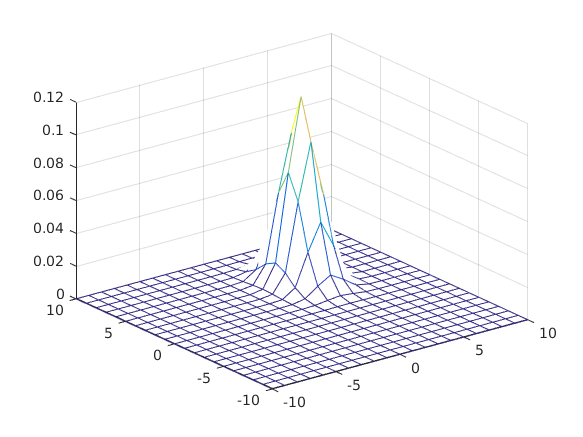
\includegraphics[width=.7\textwidth]{Ass31.png}
 \caption{Two-dimensional Gaussian pdf plotted on a mesh.}
 \label{31}
\end{figure}

\subsection{2D Gaussian pdf, Mahalanobis distance}
We determined the Mahalanobis distances using the following definition:
\begin{equation}
r^2=(x-\mu)\Sigma^{-1}(x-\mu)'
\end{equation}
This yielded the following distances for the given points:
\begin{lstlisting}
>> ([10 10]-mean)*inv(cov)*([10 10]-mean).'
ans =    67
>> ([0   0]-mean)*inv(cov)*([0   0]-mean).'
ans =    17
>> ([3   4]-mean)*inv(cov)*([3   4]-mean).'
ans =     0
>> ([6   8]-mean)*inv(cov)*([6   8]-mean).'
ans =    17
\end{lstlisting}

\subsection{Independent identically distributed random binary variables}
The code in the appendix yields the following plot:

\section{2D Gaussian pdf, Mahalanobis distance}
\subsection{}
Using the code given in the appendix, we generated the following plot:
\begin{figure}[H]
 \centering
 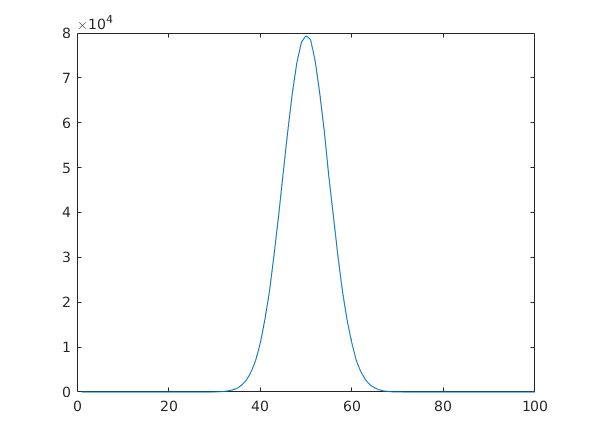
\includegraphics[width=.7\textwidth]{Ass4.png}
 \caption{Two-dimensional Gaussian pdf plotted on a mesh.}
 \label{4}
\end{figure}

This plot resembles the binomial distribution with a sequence of 100 experiments and a probability of 0.5. 
Each person that tosses a coin 100 times can be viewed as a random draw
from the binomial distribution with a probability P of 0.5 because of the 50/50 chances of the coin flip.
The 1000000 people together form 1000000 draws from this binomial
distribution, and by plotting them, an approximation of the distribution
is displayed.

By tossing a coin 100 times (N) with a 50\% chance to go forward (P),
the theoretical mean would be N*P or 100*0.5 = 50.
The variance would be N*P(1-P) = 100*0.5(1-0.5) = 25.

\subsection{Multivariate normal density, discriminant functions, minimum error rate classification, unequal priors, dichotomizer}



\subsection{Naive Bayesian rule}
Following the Naive Bayes rules as shown on the slides (so calculating the ratio):

\subsubsection{``We offer our dear customers a wide selection of classy watches''}
\begin{align}
\frac{P(spam|Customers,Watches)}{P(non-spam|Customers,Watches)}
 & = \frac{p(customers|spam)}{p(customers|non-spam)} \frac{p(watches|spam)}{p(watches|non-spam)} \frac{p(spam)}{p(non-spam)} \\
 & = \frac{0.005*0.0003*0.9}{0.0001*0.000004*0.1} \\
 & = 33750
\end{align}
So with a ratio of 33750:1 (spam:non-spam) it is very likely that the message can be classified as spam (a probability of approximately 0.99997037037).

\subsubsection{``Did you have fun on vacation? I sure did!''}
\begin{align}
\frac{P(spam|Fun,Vacation)}{P(non-spam|Fun,Vacation)}
& = \frac{p(fun|spam)}{p(fun|non-spam)} \frac{p(vacation|spam)}{p(vacation|non-spam)} \frac{p(spam)}{p(non-spam)} \\
& = \frac{0.00015*0.00025*0.9}{0.0007*0.00014*0.1} \\
& = 3.4439
\end{align}
So with a ratio of 3.4439:1 (spam:non-spam) it is likely that the message can be classified as spam (with a probability of approximately 0.7096315224).

\section*{Appendix}
\subsection*{Code for assignment 1}
\begin{lstlisting}
v1 = [4,5,6];
v2 = [6,3,9];
v3 = [8,7,3];
v4 = [7,4,8];
v5 = [4,6,5];

m1 = [v1;v2;v3;v4;v5];

mean1 = [mean(m1(:,1)); mean(m1(:,2)); mean(m1(:,3))];

cov1 = cov(m1);

mean1
cov1
\end{lstlisting}

\subsection*{Code for assignment 3}
\begin{lstlisting}
% Generate a two-dimensional Gaussian pdf with a mean [3 4] and covariance matrix  
% 1 0
% 0 2
mean = [3 4]
cov = [1 0; 0 2]
dist = gmdistribution(mean,cov)

inputmatrix = [0 0];

counter = 1;
for i = -10:10
    for j = -10:10
        inputmatrix(counter,:) = [i j];
        
        counter = counter + 1;
    end
end
% 1. Plot this function on [-10 10] x [-10 10]Using the mesh function.
output = reshape(pdf(dist, inputmatrix),[21,21])
mesh(-10:10,-10:10,output) % 
\end{lstlisting}

\subsection*{Code for assignment 4}
\begin{lstlisting}
output = zeros(100,1);
for i=1:1000000
    step = 0;
    for j = 1:100
        if rand > 0.5
            % Move forward
            step = step + 1;
        end
    end
    output(step) = output(step) + 1;
end

plot(output)
\end{lstlisting}


\end{document}
